\hypertarget{problem_8c}{
\section{lib/problem.c File Reference}
\label{problem_8c}\index{lib/problem.c@{lib/problem.c}}
}
Functions for working with problem data. 

{\tt \#include \char`\"{}arrow.h\char`\"{}}\par


Include dependency graph for problem.c:\nopagebreak
\begin{figure}[H]
\begin{center}
\leavevmode
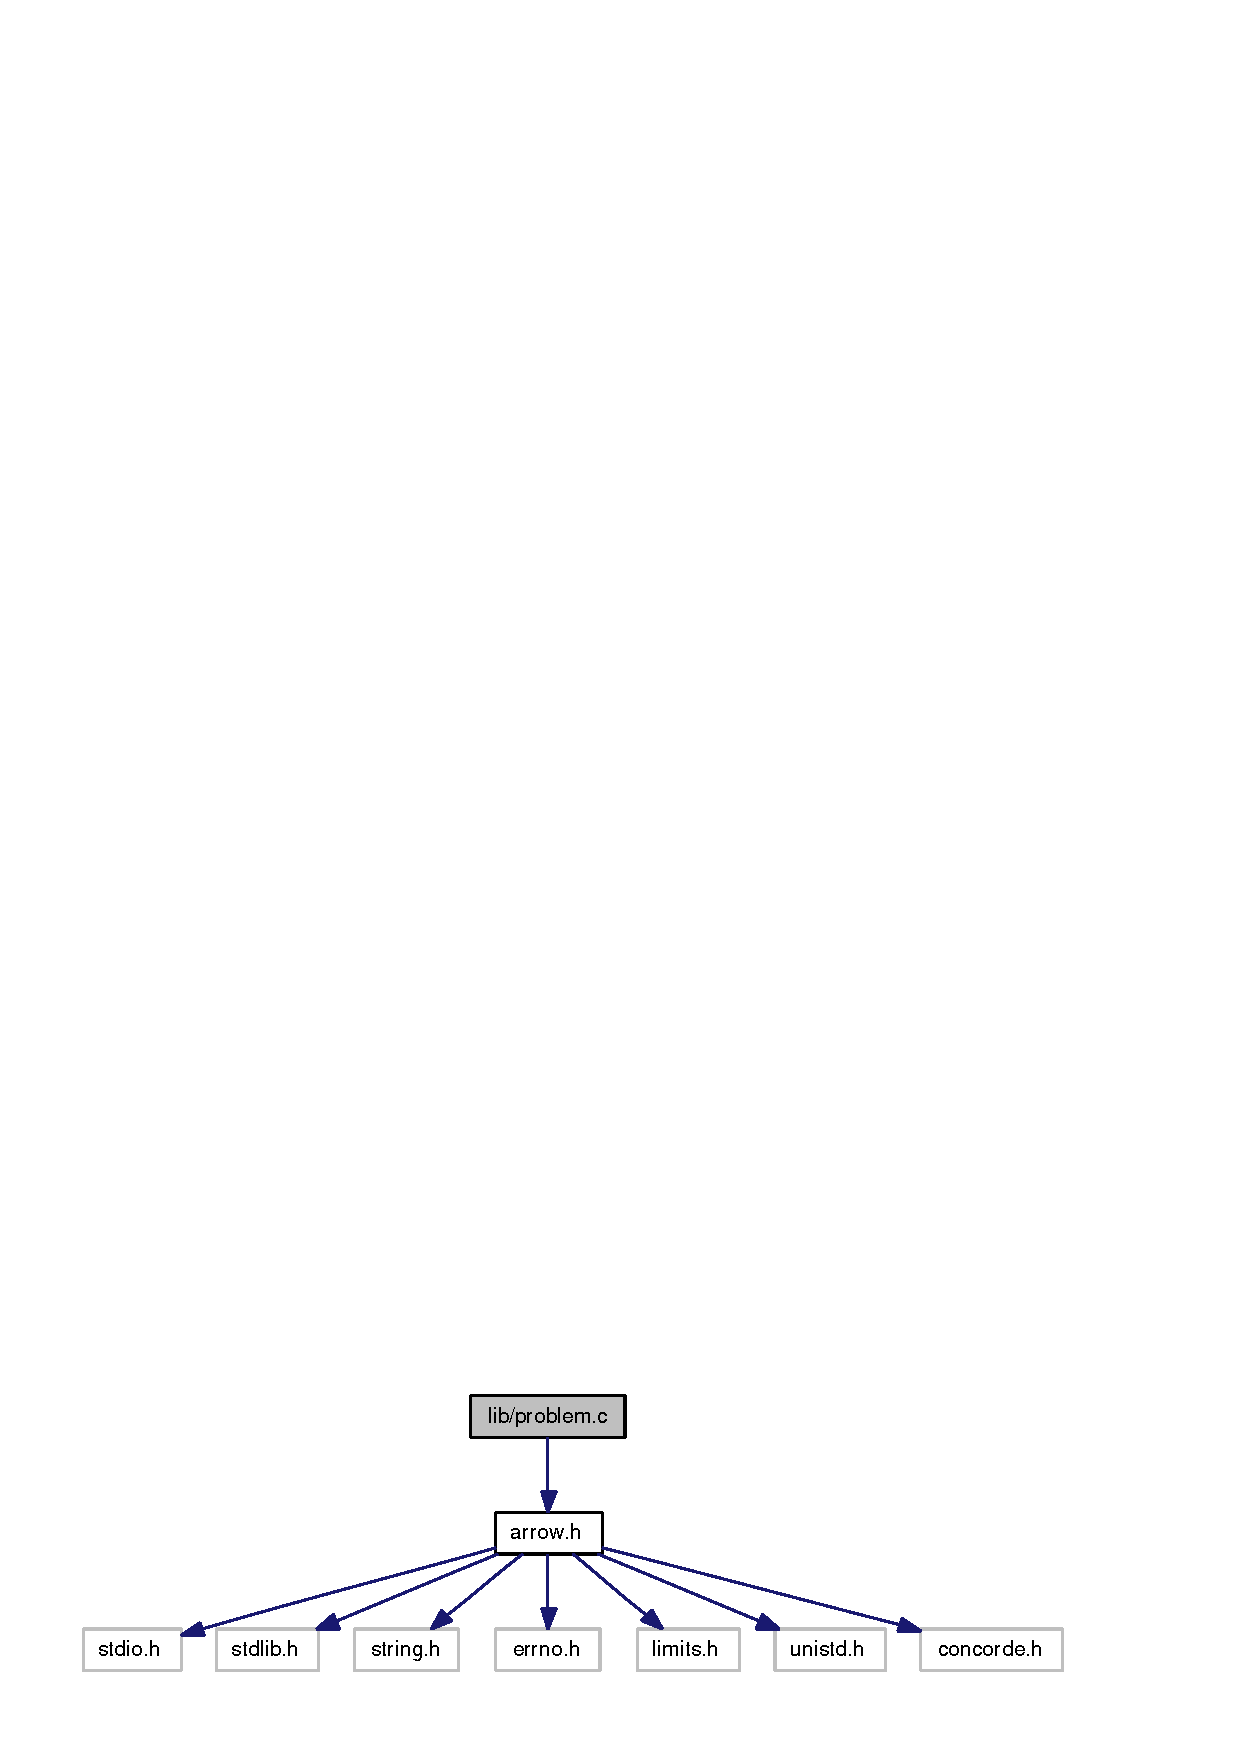
\includegraphics[width=257pt]{problem_8c__incl}
\end{center}
\end{figure}
\subsection*{Functions}
\begin{CompactItemize}
\item 
int \hyperlink{problem_8c_a634c4ee36960c1a0d23addc8bc79fb3}{concorde\_\-get\_\-cost} (\hyperlink{structarrow__problem}{arrow\_\-problem} $\ast$problem, int i, int j)
\begin{CompactList}\small\item\em Retrieves cost from Concorde data structure. \item\end{CompactList}\item 
int \hyperlink{problem_8c_b5b9bae9f92630983d3b3d39d86198f8}{arrow\_\-problem\_\-read} (char $\ast$file\_\-name, \hyperlink{structarrow__problem}{arrow\_\-problem} $\ast$problem)
\begin{CompactList}\small\item\em Reads a problem from a TSPLIB file. \item\end{CompactList}\item 
void \hyperlink{problem_8c_a702972ab510dcc6354d7679759611d1}{arrow\_\-problem\_\-destruct} (\hyperlink{structarrow__problem}{arrow\_\-problem} $\ast$problem)
\begin{CompactList}\small\item\em Deallocates problem data structure. \item\end{CompactList}\item 
int \hyperlink{problem_8c_01623c45a7e1726ef7eeeec300e75bff}{arrow\_\-problem\_\-info\_\-get} (\hyperlink{structarrow__problem}{arrow\_\-problem} $\ast$problem, \hyperlink{structarrow__problem__info}{arrow\_\-problem\_\-info} $\ast$info)
\begin{CompactList}\small\item\em Builds ordered cost list and finds min/max cost in a problem. \item\end{CompactList}\item 
void \hyperlink{problem_8c_09a5ba81556412e281fe6b863a6f08db}{arrow\_\-problem\_\-info\_\-destruct} (\hyperlink{structarrow__problem__info}{arrow\_\-problem\_\-info} $\ast$info)
\begin{CompactList}\small\item\em Deallocates problem info data structure. \item\end{CompactList}\item 
void \hyperlink{problem_8c_ce6b857eab0a7a887262d033b7e5cf22}{arrow\_\-problem\_\-print} (\hyperlink{structarrow__problem}{arrow\_\-problem} $\ast$problem)
\begin{CompactList}\small\item\em Prints out information about a problem. \item\end{CompactList}\end{CompactItemize}


\subsection{Detailed Description}
Functions for working with problem data. 

Function implemenations for working with problem data, generally manipulating the \hyperlink{structarrow__problem}{arrow\_\-problem} data structure.

\begin{Desc}
\item[Author:]John LaRusic \end{Desc}


Definition in file \hyperlink{problem_8c-source}{problem.c}.

\subsection{Function Documentation}
\hypertarget{problem_8c_a702972ab510dcc6354d7679759611d1}{
\index{problem.c@{problem.c}!arrow\_\-problem\_\-destruct@{arrow\_\-problem\_\-destruct}}
\index{arrow\_\-problem\_\-destruct@{arrow\_\-problem\_\-destruct}!problem.c@{problem.c}}
\subsubsection{\setlength{\rightskip}{0pt plus 5cm}void arrow\_\-problem\_\-destruct ({\bf arrow\_\-problem} $\ast$ {\em problem})}}
\label{problem_8c_a702972ab510dcc6354d7679759611d1}


Deallocates problem data structure. 

\begin{Desc}
\item[Parameters:]
\begin{description}
\item[{\em problem}]\mbox{[}in\mbox{]} problem data structure \end{description}
\end{Desc}


Definition at line 50 of file problem.c.

References arrow\_\-problem::data.

Referenced by main().\hypertarget{problem_8c_09a5ba81556412e281fe6b863a6f08db}{
\index{problem.c@{problem.c}!arrow\_\-problem\_\-info\_\-destruct@{arrow\_\-problem\_\-info\_\-destruct}}
\index{arrow\_\-problem\_\-info\_\-destruct@{arrow\_\-problem\_\-info\_\-destruct}!problem.c@{problem.c}}
\subsubsection{\setlength{\rightskip}{0pt plus 5cm}void arrow\_\-problem\_\-info\_\-destruct ({\bf arrow\_\-problem\_\-info} $\ast$ {\em info})}}
\label{problem_8c_09a5ba81556412e281fe6b863a6f08db}


Deallocates problem info data structure. 

\begin{Desc}
\item[Parameters:]
\begin{description}
\item[{\em info}]\mbox{[}in\mbox{]} problem info data structure \end{description}
\end{Desc}


Definition at line 99 of file problem.c.

References arrow\_\-problem\_\-info::cost\_\-list.

Referenced by main().\hypertarget{problem_8c_01623c45a7e1726ef7eeeec300e75bff}{
\index{problem.c@{problem.c}!arrow\_\-problem\_\-info\_\-get@{arrow\_\-problem\_\-info\_\-get}}
\index{arrow\_\-problem\_\-info\_\-get@{arrow\_\-problem\_\-info\_\-get}!problem.c@{problem.c}}
\subsubsection{\setlength{\rightskip}{0pt plus 5cm}int arrow\_\-problem\_\-info\_\-get ({\bf arrow\_\-problem} $\ast$ {\em problem}, \/  {\bf arrow\_\-problem\_\-info} $\ast$ {\em info})}}
\label{problem_8c_01623c45a7e1726ef7eeeec300e75bff}


Builds ordered cost list and finds min/max cost in a problem. 

\begin{Desc}
\item[Parameters:]
\begin{description}
\item[{\em problem}]\mbox{[}in\mbox{]} problem data structure \item[{\em info}]\mbox{[}out\mbox{]} problem info data structure \end{description}
\end{Desc}


Definition at line 60 of file problem.c.

References arrow\_\-bintree\_\-destruct(), arrow\_\-bintree\_\-init(), arrow\_\-bintree\_\-insert(), arrow\_\-bintree\_\-to\_\-array(), ARROW\_\-SUCCESS, arrow\_\-problem\_\-info::cost\_\-list, arrow\_\-problem\_\-info::cost\_\-list\_\-length, arrow\_\-problem::get\_\-cost, arrow\_\-problem\_\-info::max\_\-cost, arrow\_\-problem\_\-info::min\_\-cost, arrow\_\-bintree::size, and arrow\_\-problem::size.

Referenced by main().\hypertarget{problem_8c_ce6b857eab0a7a887262d033b7e5cf22}{
\index{problem.c@{problem.c}!arrow\_\-problem\_\-print@{arrow\_\-problem\_\-print}}
\index{arrow\_\-problem\_\-print@{arrow\_\-problem\_\-print}!problem.c@{problem.c}}
\subsubsection{\setlength{\rightskip}{0pt plus 5cm}void arrow\_\-problem\_\-print ({\bf arrow\_\-problem} $\ast$ {\em problem})}}
\label{problem_8c_ce6b857eab0a7a887262d033b7e5cf22}


Prints out information about a problem. 

\begin{Desc}
\item[Parameters:]
\begin{description}
\item[{\em problem}]\mbox{[}in\mbox{]} problem data structure \end{description}
\end{Desc}


Definition at line 106 of file problem.c.

References arrow\_\-problem::get\_\-cost, and arrow\_\-problem::size.\hypertarget{problem_8c_b5b9bae9f92630983d3b3d39d86198f8}{
\index{problem.c@{problem.c}!arrow\_\-problem\_\-read@{arrow\_\-problem\_\-read}}
\index{arrow\_\-problem\_\-read@{arrow\_\-problem\_\-read}!problem.c@{problem.c}}
\subsubsection{\setlength{\rightskip}{0pt plus 5cm}int arrow\_\-problem\_\-read (char $\ast$ {\em file\_\-name}, \/  {\bf arrow\_\-problem} $\ast$ {\em problem})}}
\label{problem_8c_b5b9bae9f92630983d3b3d39d86198f8}


Reads a problem from a TSPLIB file. 

\begin{Desc}
\item[Parameters:]
\begin{description}
\item[{\em file\_\-name}]\mbox{[}in\mbox{]} path to TSPLIB file \item[{\em problem}]\mbox{[}out\mbox{]} problem data structure \end{description}
\end{Desc}


Definition at line 30 of file problem.c.

References ARROW\_\-ERROR\_\-FATAL, ARROW\_\-FALSE, ARROW\_\-SUCCESS, concorde\_\-get\_\-cost(), arrow\_\-problem::data, arrow\_\-problem::get\_\-cost, arrow\_\-problem::name, arrow\_\-problem::shallow, and arrow\_\-problem::size.

Referenced by main().\hypertarget{problem_8c_a634c4ee36960c1a0d23addc8bc79fb3}{
\index{problem.c@{problem.c}!concorde\_\-get\_\-cost@{concorde\_\-get\_\-cost}}
\index{concorde\_\-get\_\-cost@{concorde\_\-get\_\-cost}!problem.c@{problem.c}}
\subsubsection{\setlength{\rightskip}{0pt plus 5cm}int concorde\_\-get\_\-cost ({\bf arrow\_\-problem} $\ast$ {\em problem}, \/  int {\em i}, \/  int {\em j})\hspace{0.3cm}{\tt  \mbox{[}inline\mbox{]}}}}
\label{problem_8c_a634c4ee36960c1a0d23addc8bc79fb3}


Retrieves cost from Concorde data structure. 

\begin{Desc}
\item[Parameters:]
\begin{description}
\item[{\em problem}]\mbox{[}in\mbox{]} pointer to \hyperlink{structarrow__problem}{arrow\_\-problem} structure \item[{\em i}]\mbox{[}in\mbox{]} id of starting node \item[{\em j}]\mbox{[}in\mbox{]} id of ending node \end{description}
\end{Desc}
\begin{Desc}
\item[Returns:]cost between node i and node j \end{Desc}


Definition at line 155 of file problem.c.

References arrow\_\-problem::data.

Referenced by arrow\_\-problem\_\-read().